\documentclass[12pt,a4paper,oneside]{report}

\usepackage[spanish]{babel}
\usepackage{fontspec}
\setmainfont{Latin Modern Roman}
\setsansfont{Latin Modern Sans}
\setmonofont{Latin Modern Mono}
\usepackage[a4paper,margin=2.5cm,headheight=24pt,headsep=18pt]{geometry}
\usepackage{graphicx}
\usepackage{float}
\usepackage{fancyhdr}
\usepackage{enumitem}
\usepackage{xcolor}
\usepackage{listings}
\usepackage{caption}
\usepackage{xurl}
\usepackage{hyperref}
\usepackage{microtype}

\hypersetup{
  colorlinks=true,
  linkcolor=blue!45!black,
  urlcolor=blue!55!black,
  pdftitle={Guía de Laboratorio 06 - Implementación de Room Database en Kotlin},
  pdfauthor={Escuela Profesional de Ingeniería de Sistemas}
}

\definecolor{codebackground}{RGB}{246,248,251}
\definecolor{coderule}{RGB}{205,213,224}
\definecolor{codekeyword}{RGB}{35,78,130}
\definecolor{codecomment}{RGB}{90,120,95}

\lstdefinelanguage{Kotlin}{
  morekeywords={abstract,annotation,as,break,class,companion,const,continue,data,
    do,else,enum,external,false,final,for,fun,if,import,in,interface,is,lateinit,
    null,object,open,override,package,private,protected,public,return,sealed,
    super,suspend,this,throw,true,try,typealias,val,var,when,while},
  sensitive=true,
  morecomment=[l]{//},
  morecomment=[s]{/*}{*/},
  morestring=[b]"
}

\lstset{
  language=Kotlin,
  basicstyle=\ttfamily\small,
  keywordstyle=\color{codekeyword}\bfseries,
  commentstyle=\color{codecomment}\itshape,
  stringstyle=\color{red!55!black},
  backgroundcolor=\color{codebackground},
  rulecolor=\color{coderule},
  frame=single,
  breaklines=true,
  breakatwhitespace=false,
  columns=fullflexible,
  keepspaces=true,
  showstringspaces=false,
  tabsize=2,
  xleftmargin=0.4em,
  xrightmargin=0.4em,
  aboveskip=0.8em,
  belowskip=0.8em
}

\pagestyle{fancy}
\fancyhf{}
\fancyhead[L]{
\includegraphics[height=0.65cm]{figuras/sello-upt.jpg}}
\fancyhead[R]{\small Escuela Profesional de Ingeniería de Sistemas}
\fancyfoot[L]{\small Mag. Alberto Johnatan Flor Rodríguez}
\fancyfoot[R]{\thepage}
\renewcommand{\headrulewidth}{0.4pt}
\renewcommand{\footrulewidth}{0pt}
\setlength{\parskip}{0.45em}
\setlength{\parindent}{0pt}
\setlength{\emergencystretch}{2em}
\setcounter{tocdepth}{2}

\begin{document}

\begin{titlepage}
\thispagestyle{empty}
\centering
\vspace*{0.5cm}
{\Large\bfseries UNIVERSIDAD PRIVADA DE TACNA\par}
\vspace{0.2cm}
{\large FACULTAD DE INGENIERÍA\par}
{\large ESCUELA DE INGENIERÍA DE SISTEMAS\par}
\vspace{1.0cm}

\includegraphics[width=3.4cm]{figuras/logo-epis.png}\par
\vspace{0.8cm}
{\Large\bfseries Guía Práctica de Laboratorio\par}
\vspace{0.4cm}
{\LARGE\bfseries Implementación de Room Database en Kotlin\par}
\vspace{1.0cm}
{\large Que se presenta para el curso:\par}
{\large\bfseries SOLUCIONES MÓVILES I\par}
\vspace{1.0cm}
{\large\bfseries AUTOR(ES):\par}
{\large APELLIDOS Y NOMBRES\par}
\vspace{0.6cm}
{\large Docente:\par}
{\large Mag. Alberto Johnatan Flor Rodríguez\par}
\vfill
{\large TACNA -- PERÚ\par}
{\large 2026\par}
\end{titlepage}

\pagenumbering{roman}
\tableofcontents
\clearpage
\pagenumbering{arabic}

\chapter*{Introducción}
\addcontentsline{toc}{chapter}{Introducción}

En el desarrollo de aplicaciones Android modernas, la persistencia de datos es un
pilar fundamental para ofrecer una experiencia de usuario fluida, permitiendo que
la información se mantenga disponible incluso sin conexión a internet o tras cerrar
la aplicación. Room Database se presenta como una capa de abstracción sobre
SQLite que facilita el acceso a la base de datos, aprovechando la potencia de SQLite
mientras proporciona verificación de consultas en tiempo de compilación.

Este laboratorio práctico se centra en la arquitectura de persistencia recomendada
por Google. Se utilizan los tres componentes clave de Room:
\begin{enumerate}[label=\arabic*.]
  \item \textbf{Entity:} representa las tablas de la base de datos.
  \item \textbf{DAO (Data Access Object):} define los métodos para acceder a los datos.
  \item \textbf{Database:} sirve como punto de acceso principal a la conexión.
\end{enumerate}

Además, se integra el uso de corrutinas de Kotlin y el componente ViewModel para
que las operaciones de entrada/salida se realicen de forma asíncrona, manteniendo
la interfaz de usuario reactiva y libre de bloqueos.

\chapter{Guía de Laboratorio No. 06: Implementación de Room Database en Kotlin}

\section{Información sobre el evento práctico}

\subsection{Título del evento práctico}
Implementación de Room Database en Kotlin.

\subsection{Objetivos}
\begin{itemize}
  \item Implementar Room como medio de almacenamiento interno de información.
  \item Integrar Workers con corrutinas mediante \texttt{Dispatchers.IO} para optimizar el uso de hilos.
\end{itemize}

\subsection{Tiempo de duración}
2 horas.

\subsection{Resultados de aprendizaje}
\begin{itemize}
  \item Gestionar tareas de larga duración fuera del hilo principal y garantizar la persistencia de procesos aunque la aplicación se cierre.
  \item Aplicar la separación de responsabilidades delegando la lógica de trabajo pesado a Workers especializados.
\end{itemize}

\subsection{Recursos}
\begin{itemize}
  \item Computadora con acceso a internet.
  \item Android Studio.
  \item Dispositivo Android físico o un Android Virtual Device (AVD).
\end{itemize}

\section{Procedimiento o metodología}

\subsection{Inicio de la aplicación}
Se crea un proyecto nuevo en Android Studio con la plantilla \textit{Empty Activity}.

\begin{figure}[H]
  \centering
  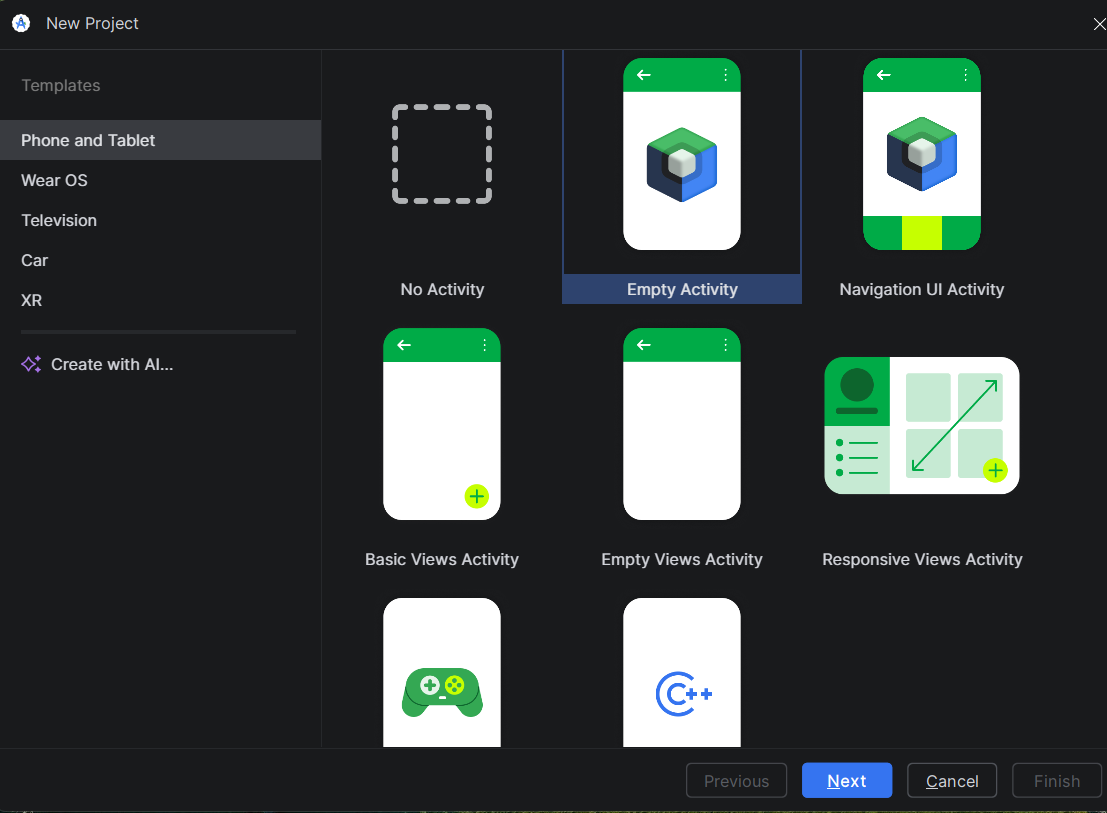
\includegraphics[width=0.78\textwidth]{figuras/android-studio-proyecto.png}
  \caption{Selección de la plantilla Empty Activity en Android Studio.}
\end{figure}

\subsection{Nombre del proyecto}
Se asigna el nombre \texttt{roomDatabase}, el paquete
\texttt{com.example.roomdatabase} y el lenguaje Kotlin.

\begin{figure}[H]
  \centering
  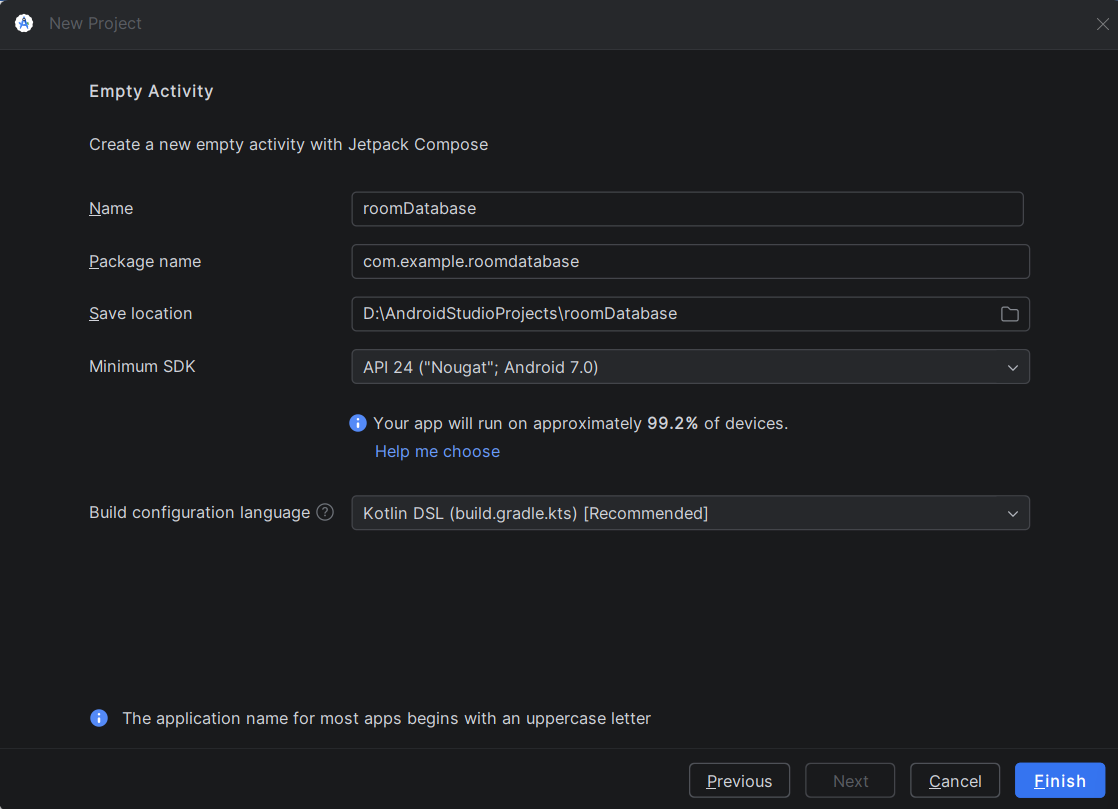
\includegraphics[width=0.82\textwidth]{figuras/android-studio-configuracion.png}
  \caption{Configuración inicial del proyecto roomDatabase.}
\end{figure}

\subsection{Clases y disposición de la aplicación}
Se propone la siguiente distribución de clases para cubrir la lógica de
mantenimiento de tablas mediante Room:

\begin{lstlisting}[language=Java]
@startuml
package "UI Layer" {
  class MainActivity {
    - viewModel: MainViewModel
    + onCreate()
  }
  class MainViewModel {
    + insertUser()
    + insertUserList()
    + updateUser()
    + deleteUser()
    + getAllUsers()
  }
}
package "Application" {
  class RoomApplication {
    {static} + db: AppDatabase
    + onCreate()
  }
}
package "Data Layer (Room)" {
  abstract class AppDatabase {
    + {abstract} userDao(): UserDao
  }
  interface UserDao <<interface>> {
    + insertUser(user: UserEntity): Long
    + insertUserList(people: List<UserEntity>): List<Long>
    + updateUser(user: UserEntity): Int
    + deleteUser(user: UserEntity): Int
    + getAll(): List<UserEntity>
    + getAllById(userIds: IntArray): List<UserEntity>
  }
  class UserEntity <<data>> {
    + userId: Int
    + nombres: String?
    + apellidos: String?
  }
}
MainActivity --> MainViewModel : usa
MainViewModel --> RoomApplication : accede db
RoomApplication o-- AppDatabase : mantiene instanciado
AppDatabase ..> UserDao : provee
UserDao ..> UserEntity : opera con
@enduml
\end{lstlisting}

\begin{figure}[H]
  \centering
  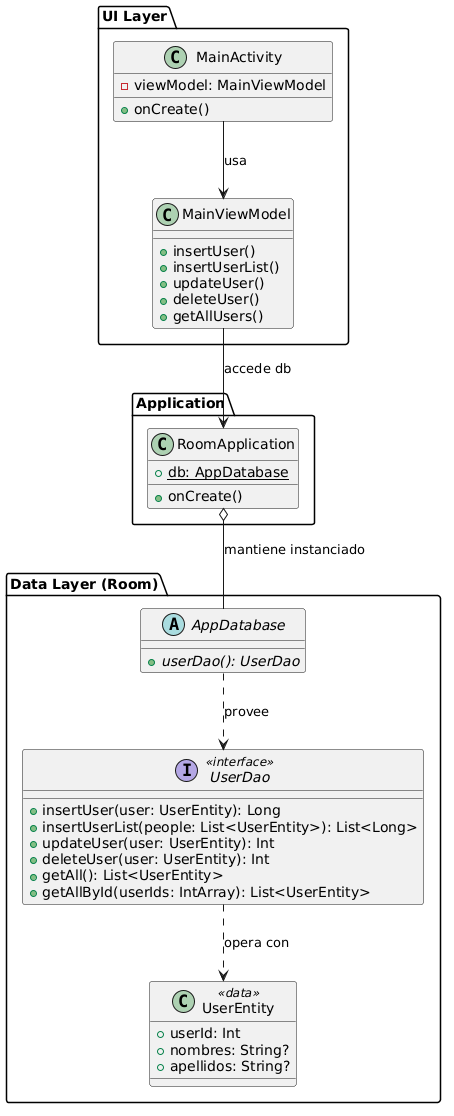
\includegraphics[height=0.76\textheight,keepaspectratio]{figuras/diagrama-clases.png}
  \caption{Diagrama de clases y relaciones de la solución base.}
\end{figure}

\subsection{Configuración de Gradle, Kotlin y KSP}
Se modifican los archivos de Gradle para configurar el compilador, KSP y las
dependencias de Room. Las versiones indicadas por la guía son Kotlin 2.3.21,
Compose BOM 2026.04.01, KSP 2.3.4 y Room 2.8.4.

\begin{lstlisting}[language=Java]
[versions]
kotlin = "2.3.21"
composeBom = "2026.04.01"
kotlinskp = "2.3.4"

[plugins]
android-application = { id = "com.android.application", version.ref = "agp" }
kotlin-compose = { id = "org.jetbrains.kotlin.plugin.compose", version.ref = "kotlin" }
kotlinksp = { id = "com.google.devtools.ksp", version.ref = "kotlinskp" }
\end{lstlisting}

En el Gradle del proyecto se declara KSP sin aplicarlo al módulo raíz:
\begin{lstlisting}
plugins {
  alias(libs.plugins.kotlinksp) apply false
}
\end{lstlisting}

En el Gradle de la aplicación se aplica el plugin y se agregan las dependencias:
\begin{lstlisting}
plugins {
  alias(libs.plugins.kotlinksp)
}

dependencies {
  val room_version = "2.8.4"
  implementation("androidx.room:room-runtime:$room_version")
  ksp("androidx.room:room-compiler:$room_version")
  annotationProcessor("androidx.room:room-compiler:$room_version")
  implementation("androidx.room:room-ktx:$room_version")
}
\end{lstlisting}

Se crean los paquetes principales: \texttt{application}; \texttt{data}, con los
subpaquetes \texttt{dao}, \texttt{database} y \texttt{entity}; además de
\texttt{ui} y \texttt{viewmodel}.

\begin{figure}[H]
  \centering
  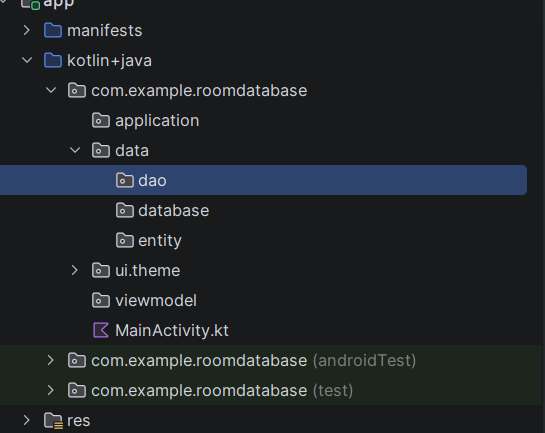
\includegraphics[width=0.55\textwidth]{figuras/estructura-paquetes.png}
  \caption{Estructura de paquetes mostrada en Android Studio en la guía original.}
\end{figure}

\subsection{Entidad UserEntity}
La entidad representa la tabla \texttt{users}. El identificador se genera
automáticamente y los campos de nombre se guardan en columnas con nombres
explícitos.

\begin{lstlisting}
package com.example.roomdatabase.data.entity

import androidx.room.ColumnInfo
import androidx.room.Entity
import androidx.room.PrimaryKey

@Entity(tableName = "users")
data class UserEntity(
  @PrimaryKey(autoGenerate = true) val userId: Int = 0,
  @ColumnInfo(name = "first_name") val nombres: String?,
  @ColumnInfo(name = "last_name") val apellidos: String?
)
\end{lstlisting}

\subsection{DAO}
La interfaz \texttt{UserDao} define las operaciones de inserción, actualización,
eliminación y consulta:

\begin{lstlisting}
package com.example.roomdatabase.data.dao

import androidx.room.Dao
import androidx.room.Delete
import androidx.room.Insert
import androidx.room.OnConflictStrategy
import androidx.room.Query
import androidx.room.Update
import com.example.roomdatabase.data.entity.UserEntity

@Dao
interface UserDao {
  @Insert(onConflict = OnConflictStrategy.ABORT)
  suspend fun insertUser(user: UserEntity): Long

  @Insert(onConflict = OnConflictStrategy.ABORT)
  suspend fun insertUserList(people: List<UserEntity>): List<Long>

  @Update
  suspend fun updateUser(user: UserEntity): Int

  @Delete
  suspend fun deleteUser(user: UserEntity): Int

  @Query("SELECT * FROM users")
  suspend fun getAll(): List<UserEntity>

  @Query("SELECT * FROM users WHERE userId IN (:userIds)")
  suspend fun getAllById(userIds: IntArray): List<UserEntity>?
}
\end{lstlisting}

\subsection{Base de datos e instancia de aplicación}
\texttt{AppDatabase} registra la entidad y ofrece acceso al DAO:
\begin{lstlisting}
@Database(entities = [UserEntity::class], version = 1)
abstract class AppDatabase : RoomDatabase() {
  abstract fun userDao(): UserDao
}
\end{lstlisting}

La clase que hereda de \texttt{Application} crea la instancia de la base de datos:
\begin{lstlisting}
class RoomApplication : Application() {
  companion object {
    lateinit var db: AppDatabase
  }

  override fun onCreate() {
    super.onCreate()
    db = Room.databaseBuilder(
      applicationContext,
      AppDatabase::class.java,
      "database-users"
    ).build()
  }
}
\end{lstlisting}

\subsection{AndroidManifest.xml}
Se indica la clase \texttt{RoomApplication} en el manifiesto:
\begin{lstlisting}[language=XML]
<application
  android:name=".application.RoomApplication"
  android:allowBackup="true"
  android:label="@string/app_name"
  android:supportsRtl="true"
  android:theme="@style/Theme.RoomDatabase">
  <activity
    android:name=".MainActivity"
    android:exported="true">
    <intent-filter>
      <action android:name="android.intent.action.MAIN" />
      <category android:name="android.intent.category.LAUNCHER" />
    </intent-filter>
  </activity>
</application>
\end{lstlisting}

\subsection{ViewModel y corrutinas}
El ViewModel ejecuta las operaciones de base de datos dentro de
\texttt{viewModelScope} y \texttt{Dispatchers.IO}. El ejemplo inserta un usuario y
un lote de cinco usuarios:
\begin{lstlisting}
class MainViewModel : ViewModel() {
  fun insertUser() {
    val user = UserEntity(nombres = "Juan", apellidos = "Perez")
    viewModelScope.launch(Dispatchers.IO) {
      RoomApplication.db.userDao().insertUser(user)
    }
  }

  fun insertUserList() {
    val users = listOf(
      UserEntity(nombres = "Juan", apellidos = "Perez"),
      UserEntity(nombres = "Maria", apellidos = "Lopez"),
      UserEntity(nombres = "Pedro", apellidos = "Gonzalez"),
      UserEntity(nombres = "Ana", apellidos = "Martinez"),
      UserEntity(nombres = "Luis", apellidos = "Garcia")
    )
    viewModelScope.launch(Dispatchers.IO) {
      RoomApplication.db.userDao().insertUserList(users)
    }
  }
}
\end{lstlisting}

La actividad obtiene el ViewModel con \texttt{by viewModels()} y, en la solución
base de la guía, invoca sus operaciones desde \texttt{onCreate()}.

\subsection{Actualización, eliminación y consulta}
Los métodos restantes de mantenimiento actualizan, eliminan y consultan usuarios:
\begin{lstlisting}
fun updateUser() {
  val user = UserEntity(userId = 1, nombres = "Jorge", apellidos = "Perez")
  viewModelScope.launch(Dispatchers.IO) {
    RoomApplication.db.userDao().updateUser(user)
    println("DEBUG: Usuario actualizado correctamente")
  }
}

fun deleteUser() {
  val user = UserEntity(userId = 4, nombres = "", apellidos = "")
  viewModelScope.launch(Dispatchers.IO) {
    RoomApplication.db.userDao().deleteUser(user)
  }
}

fun getAllUsers() {
  viewModelScope.launch(Dispatchers.IO) {
    val users = RoomApplication.db.userDao().getAll()
    users.forEach { user ->
      println("DEBUG: $user")
    }
  }
}
\end{lstlisting}

\chapter{Ampliación implementada}

\section{Enunciado}
Una vez implementada la estructura básica de \texttt{UserEntity} y su
mantenimiento, se escala la aplicación para que sea funcional para un usuario
final, añadiendo validaciones y una visualización de datos más robusta.

\begin{enumerate}
  \item \textbf{Modificación de la entidad.}
  Agregar el campo nullable \texttt{email}; actualizar \texttt{AppDatabase} a la
  versión 2 y configurar la política de migración destructiva básica solicitada.
  \item \textbf{Búsqueda:} añadir una consulta por apellido (\texttt{last\_name})
  usando \texttt{LIKE} e implementarla en el ViewModel.
  \item \textbf{Interfaz:} crear en Jetpack Compose los campos Nombre y Apellido,
  el botón Guardar Usuario y una lista LazyColumn o RecyclerView.
  \item \textbf{Lógica de negocio:} actualizar la lista automáticamente al insertar
  o eliminar registros.
\end{enumerate}

\section{Entidad y migración}
La versión final de la entidad incorpora el correo opcional. La versión de la base
de datos es 2; al actualizar desde un esquema anterior sin una migración explícita,
la política solicitada reconstruye las tablas.

\begin{lstlisting}
@Entity(tableName = "users")
data class UserEntity(
  @PrimaryKey(autoGenerate = true) val userId: Int = 0,
  @ColumnInfo(name = "first_name") val nombres: String?,
  @ColumnInfo(name = "last_name") val apellidos: String?,
  @ColumnInfo(name = "email") val email: String? = null
)

@Database(entities = [UserEntity::class], version = 2, exportSchema = true)
abstract class AppDatabase : RoomDatabase() {
  abstract fun userDao(): UserDao
}

db = Room.databaseBuilder(
  applicationContext,
  AppDatabase::class.java,
  "database-users"
).fallbackToDestructiveMigration().build()
\end{lstlisting}

\section{Búsqueda por apellido y lista reactiva}
El DAO expone una consulta con \texttt{LIKE} como \texttt{Flow}. El ViewModel
selecciona la consulta general o la búsqueda según el texto ingresado; Room vuelve
a emitir la lista cuando cambian las filas de \texttt{users}.

\begin{lstlisting}
@Query(
  "SELECT * FROM users " +
  "WHERE last_name LIKE '%' || :query || '%' " +
  "ORDER BY userId DESC"
)
fun searchByLastName(query: String): Flow<List<UserEntity>>

val users: StateFlow<List<UserEntity>> = _lastNameQuery
  .flatMapLatest { query ->
    if (query.isBlank()) userDao.observeAll()
    else userDao.searchByLastName(query.trim())
  }
  .flowOn(Dispatchers.IO)
  .stateIn(
    viewModelScope,
    SharingStarted.WhileSubscribed(5_000),
    emptyList()
  )
\end{lstlisting}

\section{Interfaz de usuario}
La pantalla final incluye los dos campos solicitados, validación de campos vacíos,
alta y edición de usuarios, eliminación con confirmación, búsqueda por apellido y
una lista reactiva. El campo \texttt{email} permanece opcional en la entidad y no se
solicita en el formulario, que conserva los dos campos requeridos por el enunciado.

\begin{lstlisting}
OutlinedTextField(
  value = firstName,
  onValueChange = { firstName = it },
  label = { Text("Nombre") },
  singleLine = true
)
OutlinedTextField(
  value = lastName,
  onValueChange = { lastName = it },
  label = { Text("Apellido") },
  singleLine = true
)
Button(onClick = {
  viewModel.saveUser(firstName, lastName)
}) {
  Text("Guardar Usuario")
}
LazyColumn {
  items(items = users, key = { it.userId }) { user ->
    UserCard(user = user, onEdit = { /* cargar usuario */ },
      onDelete = { /* eliminar usuario */ })
  }
}
\end{lstlisting}

\section{Worker demostrativo}
Los objetivos y resultados de aprendizaje de la guía mencionan Workers, aunque el
procedimiento original no especifica una tarea concreta. Para cubrir ese objetivo,
se añadió el botón \textbf{Cargar lote de ejemplo con WorkManager}. Este encola un
\texttt{CoroutineWorker} idempotente que inserta los cinco usuarios de ejemplo en
\texttt{Dispatchers.IO}; la lista observada por Room se actualiza al completar la
operación.

\section{Capturas de la implementación nueva}
Las capturas se tomaron desde un AVD Pixel 7 Pro después de compilar e instalar la
app de depuración. La primera muestra la pantalla y los registros locales; la
segunda demuestra el filtro por apellido \texttt{Lopez}.

\begin{figure}[H]
  \centering
  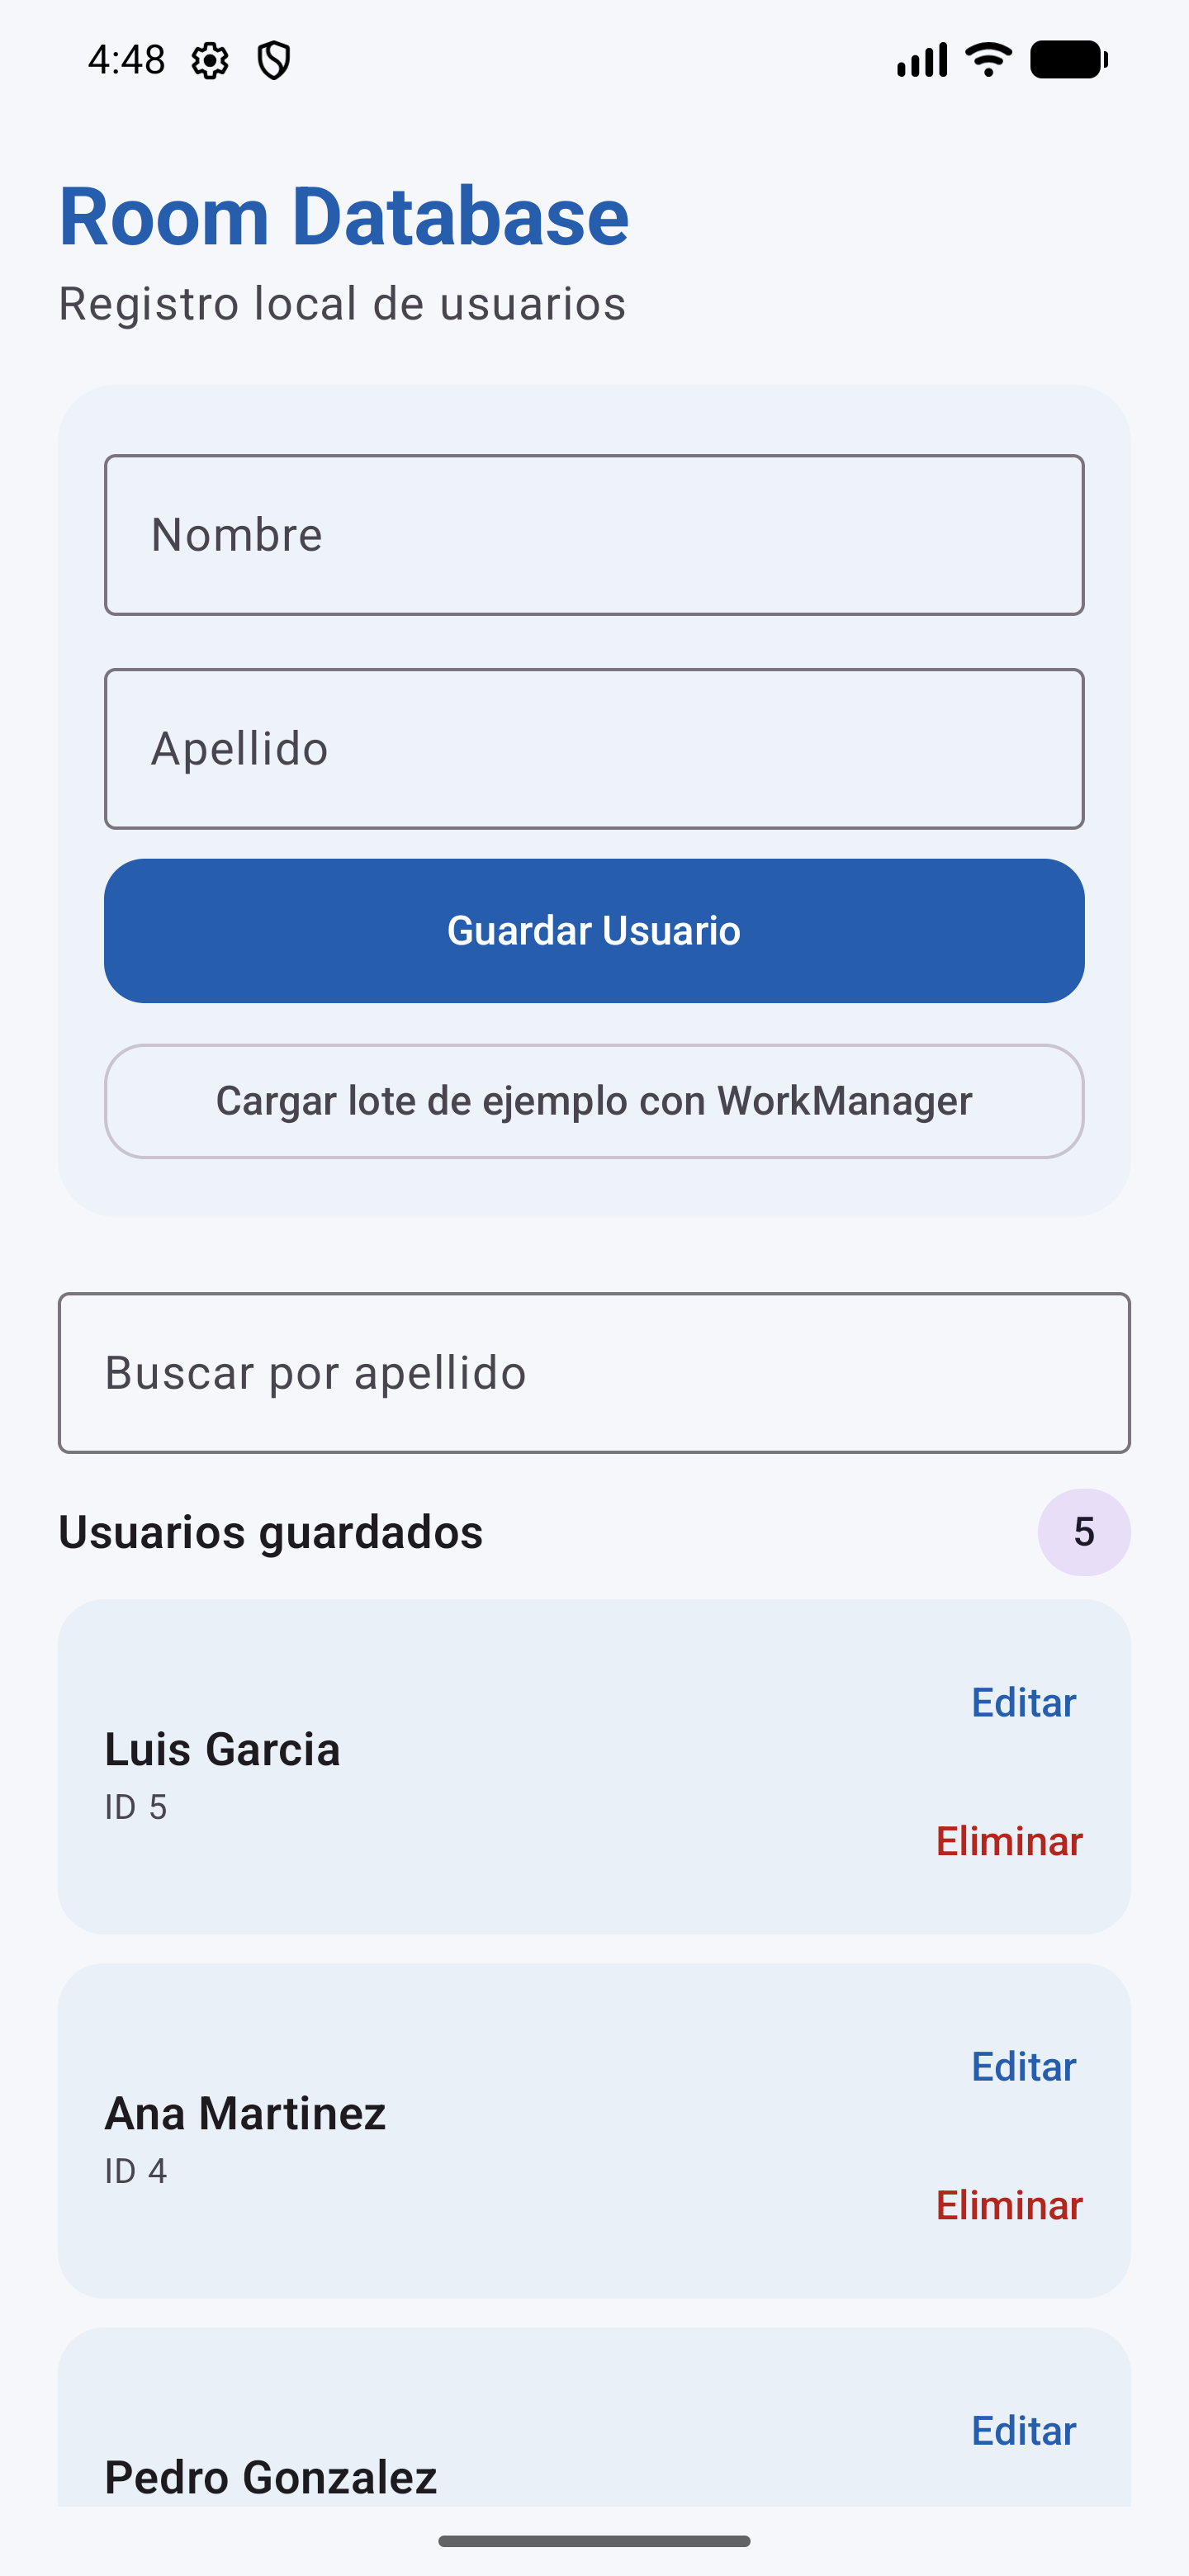
\includegraphics[height=0.69\textheight,keepaspectratio]{capturas/01-aplicacion.png}
  \caption{Pantalla Compose con usuarios guardados en Room y acciones de edición y eliminación.}
\end{figure}

\begin{figure}[H]
  \centering
  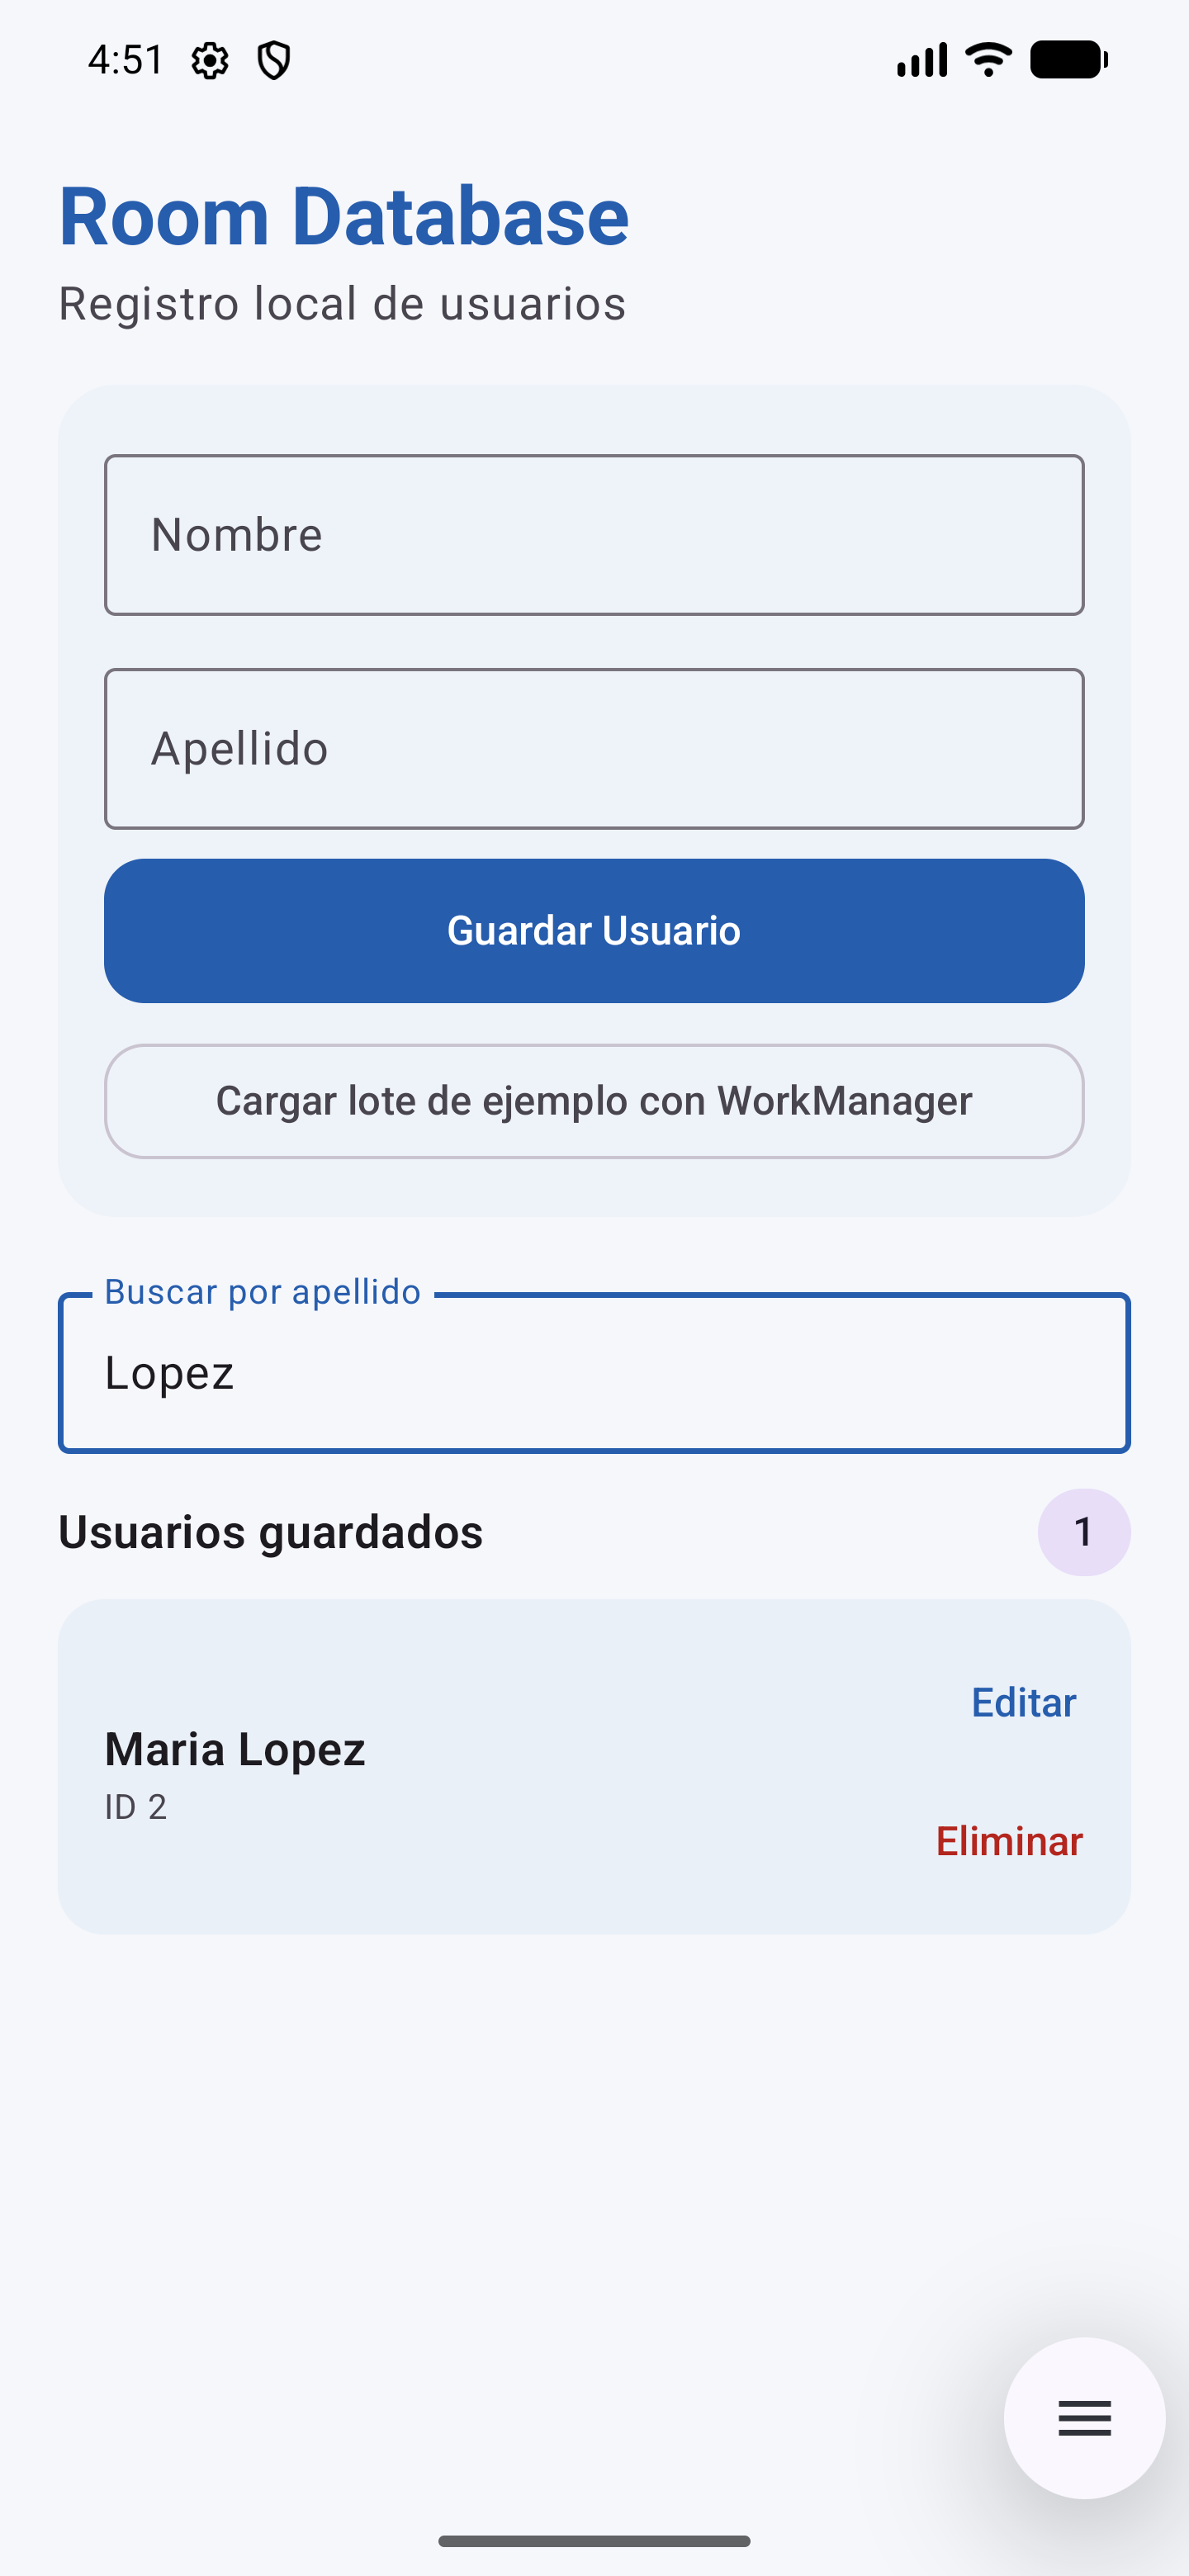
\includegraphics[height=0.69\textheight,keepaspectratio]{capturas/02-busqueda-apellido.png}
  \caption{Búsqueda reactiva por apellido: al buscar Lopez se muestra el usuario coincidente.}
\end{figure}

\chapter{Conclusiones}
\begin{enumerate}
  \item Room permite separar la representación de datos, las operaciones de acceso
  y la configuración de la base de datos mediante Entity, DAO y Database. También
  genera el código del DAO y valida las consultas durante la compilación.
  \item El uso de un \texttt{Flow} desde Room permite que Compose observe los cambios
  de la tabla y actualice la lista al insertar, actualizar o eliminar usuarios.
  \item El alcance de corrutinas del ViewModel vincula las operaciones a su ciclo
  de vida, y el dispatcher de entrada/salida mantiene el trabajo de base de datos
  fuera del hilo principal.
  \item La migración destructiva permite aplicar rápidamente el cambio al esquema
  de versión 2; en una app que deba conservar los datos existentes se debe definir
  una migración explícita.
\end{enumerate}

\chapter{Cuestionario}

\section*{1. Función de \texttt{@Dao}}
\addcontentsline{toc}{section}{1. Función de @Dao}
\texttt{@Dao} identifica una interfaz o clase que declara las operaciones para
insertar, actualizar, eliminar o consultar datos. Room genera su implementación en
compilación y valida las consultas SQL. Frente a usar directamente
\texttt{SQLiteOpenHelper}, reduce código repetitivo y permite encontrar errores de
consulta durante la compilación.

\section*{2. Clave primaria autogenerada con valor 0}
\addcontentsline{toc}{section}{2. Clave primaria autogenerada con valor 0}
Con \texttt{@PrimaryKey(autoGenerate = true)} y una clave de tipo \texttt{Int},
Room trata el valor \texttt{0} como “sin asignar”. SQLite genera un identificador
único al insertar la fila y el registro queda guardado con ese identificador.

\section*{3. DAO, ViewModel y Dispatchers.IO}
\addcontentsline{toc}{section}{3. DAO, ViewModel y Dispatchers.IO}
\texttt{viewModelScope} vincula el trabajo al ciclo de vida del ViewModel.
\texttt{Dispatchers.IO} está diseñado para tareas de entrada/salida, como leer y
escribir en almacenamiento. Si se ejecutara una operación bloqueante en el hilo
principal, la interfaz podría congelarse y Android podría mostrar un ANR. Las
funciones suspend de Room son seguras para orquestarse desde corrutinas; el
laboratorio usa \texttt{Dispatchers.IO} explícitamente para mantener clara la
separación del trabajo de base de datos.

\section*{4. Propósito de heredar de \texttt{Application}}
\addcontentsline{toc}{section}{4. Propósito de Application}
\texttt{Application} permite mantener estado compartido durante la vida del proceso
de la aplicación y su \texttt{onCreate()} se ejecuta antes de crear las actividades.
\texttt{RoomApplication} inicializa una instancia de \texttt{AppDatabase} con el
contexto de aplicación para que los componentes puedan acceder al mismo punto de
entrada.

\section*{5. Función de KSP con Room}
\addcontentsline{toc}{section}{5. Función de KSP con Room}
KSP (Kotlin Symbol Processing) procesa anotaciones y símbolos Kotlin durante la
compilación. Room lo utiliza para analizar \texttt{UserEntity}, \texttt{UserDao} y
\texttt{AppDatabase}, generar la implementación de acceso a datos y detectar
inconsistencias de consultas antes de ejecutar la aplicación.

\chapter{Comprobación de compilación}
Se compiló la variante de depuración con:
\begin{lstlisting}[language=Java]
.\gradlew.bat :app:assembleDebug
\end{lstlisting}

Resultado: \texttt{BUILD SUCCESSFUL}. El APK de depuración se genera en:
\path{app/build/outputs/apk/debug/app-debug.apk}.
La aplicación se instaló y se abrió en el AVD Pixel 7 Pro; se comprobó que el
Worker carga el lote de usuarios y que la búsqueda por apellido filtra la lista.

\chapter{Referencias bibliográficas}
\begingroup\sloppy
\begin{enumerate}
  \item Android Developers (2026). \textit{Ciclo de vida de la actividad}.
  \url{https://developer.android.com/guide/components/activities/activity-lifecycle}
  \item Android Developers (2026). \textit{Guía de WorkManager: programación de tareas asíncronas}.
  \url{https://developer.android.com/develop/background-work/background-tasks/persistent/getting-started}
  \item Kotlin Foundation (2025). \textit{Coroutines Guide: Dispatchers and Context}.
  \url{https://kotlinlang.org/docs/coroutines-basics.html}
  \item Android Developers (2026). \textit{Common Architecture Patterns: MVVM}.
  \url{https://developer.android.com/topic/architecture}
  \item Android Developers (2026). \textit{Room: guardar datos en una base de datos local}.
  \url{https://developer.android.com/training/data-storage/room}
  \item Android Developers (2026). \textit{Migrar de kapt a KSP}.
  \url{https://developer.android.com/build/migrate-to-ksp}
\end{enumerate}
\endgroup

\end{document}
